\section{Data Samples}\label{sec:DataSamples}
The data samples used for this calibration span Run-I and Run-II. The details of all the data samples are outlined in \href{https://docs.google.com/spreadsheets/d/1_0kNCKBIIx53f6vopqN2OijtcTICHD9rDvN_YKGH2mI/edit?usp=sharing}{this data production spreadsheet} and summarized in Table \ref{tab:samples}. It is worth noting, that in the inclusive pion cross-section analysis (for which a good deal of this calibration is driven by), the ``High-Yield'' beamline reconstruction is what is used to increase the statistics of the sample. Since the ``Picky Track'' reconstruction used here represents only a subset of that data, we don't use the entire measurement sample to tune our response. 

\begin{center}
\begin{table}[htb]
	\begin{center}
	%\resizebox{0.45\textwidth}{!}{%
	\begin{tabular}{c|c|c|c|c}
	\multicolumn{4}{c}{\textbf{Summary of Samples}} \\
	\hline \hline
	 Run Period & LArIATsoft Version & Beamline Reconstruction & Mass Filter & Calibration/Validation\\
	\hline
	Run-I & \verb!v06_34_01! & Negative Polarity Picky Track & $\pi, \mu, e$ & Calibration \\
	\hline
	Run-I & \verb!v06_34_01! & Negative Polarity Picky Track & Kaon & Calibration \\
	\hline
	Run-I & \verb!v06_34_01! & Positive Polarity Picky Track & $\pi, \mu, e$ & Validation \\
	\hline
	Run-I & \verb!v06_34_01! & Positive Polarity Picky Track & Kaon & Validation \\
	\hline
	Run-I & \verb!v06_34_01! & Positive Polarity Picky Track & Proton & Validation \\
	\hline
	\hline
	Run-II & \verb!v06_34_01! & Positive Polarity Picky Track & $\pi, \mu, e$ & Calibration \\
	\hline
	Run-II & \verb!v06_34_01! & Positive Polarity Picky Track & Kaon & Validation \\
	\hline
	Run-II & \verb!v06_34_01! & Positive Polarity Picky Track & Proton & Validation \\
	\hline
	Run-II & \verb!v06_34_01! & Negative Polarity Picky Track & $\pi, \mu, e$ & Validation \\
	\hline
	Run-II & \verb!v06_34_01! & Negative Polarity Picky Track & Kaon & Validation \\
	\hline
	\end{tabular}%}
	\caption{Summary of the data samples used for the calibration study. A sample listed as a ``calibration'' sample was used, tuned, checked, and re-tuned until the desired calibration was achieved. A sample listed at ``validation'' was then checked using the calorimetry constants derived for that run period. }
	\label{tab:samples}
	\end{center}
\end{table}
\end{center}

The corresponding data driven Monte Carlo (DDMC) samples which match the data samples listed in Table \ref{tab:samples} are used to tune the MC calibration constants and can be found on the data spreadsheet listed above.


%%%%%%%%%%%%%%%%%%%%%%%%%%%%%%%%%%%%%%%%%%%%%%%%%%%%%%%%%%%%
\subsection{Event Selection}\label{sec:EventSelection}
%%%%%%%%%%%%%%%%%%%%%%%%%%%%%%%%%%%%%%%%%%%%%%%%%%%%%%%%%%%%
For each sample listed in Table \ref{tab:samples}, we outline the event selection used to select this data.

\begin{itemize}
\item \textbf{Time Stamp Filter}

A filter is used to select events which occurred in time with the beam. These events typically coincide with the first 6 seconds of the beam spill, and therefore the events are filtered using the following LArIATsoft settings

\begin{verbatim}
tfilt:      @local::lariat_timestampfilter

# ====================================================================
# Specify range of events to select.  For Run I/II:
#   - pedestal events:  ~ 0.  - 1.2 sec
#   - beam events:      ~ 1.2 - 5.5 sec
#   - cosmic events:    ~ > 5.5 sec
#   (default selects ALL events)
physics.filters.tfilt.T1:                       1.2
physics.filters.tfilt.T2:                       5.5
physics.filters.tfilt.RequireRawDigits:         true

\end{verbatim}



\item \textbf{Beamline Reconstruction}

The standard LArIAT beamline reconstruction is used to select events which have a wire chamber track and TOF information in an individual event using the following modules.
\begin{verbatim}
### beamline elements ###

wctrack:     @local::lariat_wctrackbuilder
tof:         @local::lariat_tof
agcounter:   @local::lariat_aerogel
\end{verbatim}


\textbf{For Run-I we use these default parameters:}
\begin{verbatim} 
physics.producers.wctrack.PickyTracks:                          true
physics.producers.tof.HitThreshold:                           -10.0  
physics.producers.tof.HitDiffMeanUS:                            0.6  
physics.producers.tof.HitDiffMeanDS:                            1.0  
physics.producers.tof.HitMatchThresholdUS:                      3.0  
physics.producers.tof.HitMatchThresholdDS:                      6.0  
physics.producers.tof.HitWait:                                  20.
\end{verbatim}

\textbf{For Run-II we use these default parameters:}
\begin{verbatim} 
physics.producers.wctrack.PickyTracks:                          true
physics.producers.tof.HitThreshold:                             -3.
physics.producers.tof.HitDiffMeanUS:                            0.5  
physics.producers.tof.HitDiffMeanDS:                            0.4  
physics.producers.tof.HitMatchThresholdUS:                      3.0  
physics.producers.tof.HitMatchThresholdDS:                      6.0  
physics.producers.tof.HitWait:                                  20.
\end{verbatim}

\item \textbf{Particle Mass Filtering}
Using the beamline reconstruction, it is possible to calculate the mass of a given track using the following equation

\begin{equation}
mass = \frac{p}{c}\sqrt{(\frac{TOF \times c}{l})^2 -1}
\end{equation}
where $p$ represents the measured momentum from the wire chamber, $TOF$ represents the time-of-flight measured as the difference between the two time-of-flight paddles in the LArIAT beamline, $l$ is path length the particle traveled down the beamline, and $c$ represents the speed of light.

Using this it is possible to plot the mass of each track reconstructed in the particle beamline, as shown in Figure \ref{fig:mass}. The classification of events into the different samples follows:

\begin{itemize}
\item \underline{$\pi, \mu, e$:} 0~MeV $<$ mass $<$ 350~MeV

\item \underline{kaon:} 350~MeV $<$ mass $<$ 650~MeV

\item \underline{proton:} 650~MeV $<$ mass $<$ 3000~MeV

\end{itemize}

\begin{figure}[htb]
\centering
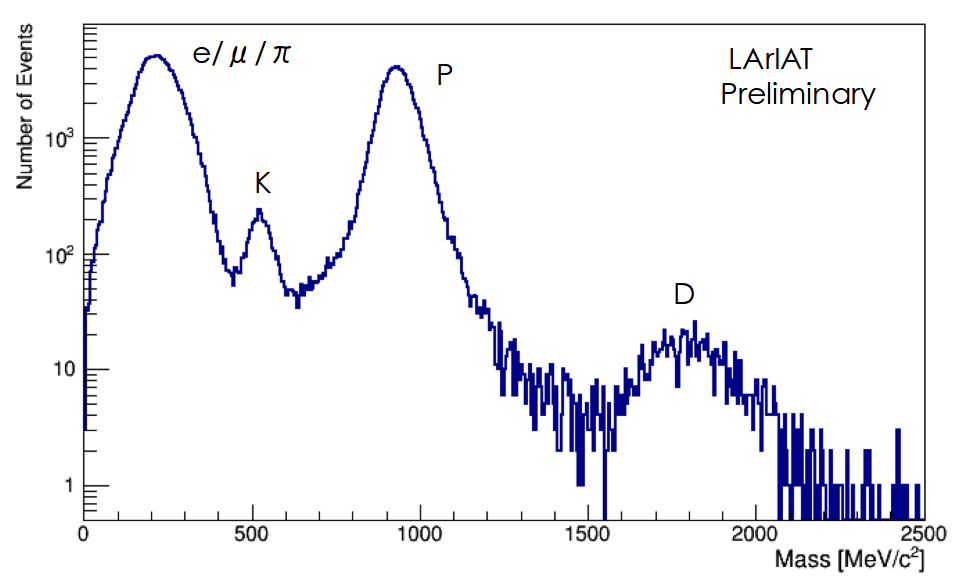
\includegraphics[width=0.70\textwidth]{images/mass.png}
\caption{The mass plotted for a sample of Run-II events reconstructed in the beamline. The classification of the events into $\pi, \mu, e$, kaon, or proton is based on this distribution.}
\label{fig:mass}
\end{figure}

\item \textbf{LArTPC Reconstruction}

Finally, events are reconstructed inside the TPC and we select events that satisfy the following requirements

\begin{itemize}
\item At least one track reconstructed inside the TPC with length $>$~10~cm
\item The event has fewer than three tracks with a length less than 5~cm reconstructed (shower veto)
\item One and only one TPC track can be matched to a wire chamber track (-4.0~cm$< \Delta X <$ 6.0~cm, -5.0~cm$< \Delta Y <$ 5.0~cm, $\alpha < 10$ degrees)

\end{itemize}


\end{itemize}

Events passing all these selection requirements are used for the dE/dX calibration. The event reduction table for all these cuts is provided in Section \ref{sec:Results} for each relevant sub-sample as well as the results from the calorimetry constant tuning.
